\documentclass[uplatex,dvipdfmx]{jsarticle}

\usepackage[dvipdfmx]{graphicx}
\usepackage[dvipdfmx]{xcolor}
\usepackage[cmex10]{amsmath}
\usepackage[deluxe]{otf}
\usepackage{booktabs}
\usepackage{ascmac}
\usepackage{amssymb}
\usepackage{caption}
\usepackage{colortbl}
\usepackage{float} 
\usepackage{textcomp}
\usepackage{url}
\usepackage{multirow,multicol}
\usepackage{wrapfig}
\usepackage{listings,jvlisting} 
\usepackage{xcolor}
\usepackage{graphicx}
\usepackage{hyperref} % \urlだけでなくリンクも有効にする場合


\lstset{
basicstyle={\ttfamily},
identifierstyle={\small},
commentstyle={\smallitshape},
keywordstyle={\small\bfseries},
ndkeywordstyle={\small},
stringstyle={\small\ttfamily}, frame={tb},
breaklines=true, columns=[l]{fullflexible},
numbers=left, xrightmargin=0zw, xleftmargin=3zw,
numberstyle={\scriptsize}, stepnumber=1,
numbersep=1zw, lineskip=-0.5ex
}

\title{期末レポート}
\author{24G1089 武本龍}
\date{2024年1月7日}

\begin{document}
\maketitle

\section{はじめに}
本報告書は,掲示板システムに「いいね機能」や「投稿時間の自動反映機能」を新たに追加した成果をまとめたものである.
利用者,管理者,開発者それぞれの視点に基づき,追加された機能の詳細な説明を行う.
さらに,利用者の利便性向上を目的としたユーザーインターフェース(UI)の工夫についても触れ,実際の使用シナリオにおいてどのように役立つかを具体的に示す.
本報告書を通じて,掲示板システムの全体像と,新機能がもたらす価値を包括的に理解できるようにすることを目指した.

\section{プログラムの概要}
今回作成したプログラムの概要を説明する.

\subsection{プログラムの保存場所}
以下のURLはGitHubのクラウド上に置かれているプログラムである.\\
https://github.com/Urban-Sea/webpro\_06

\subsection{プログラムの関係}
今回作成したプログラムの関係図を以下に示す.
\begin{figure}[h]
    \centering
    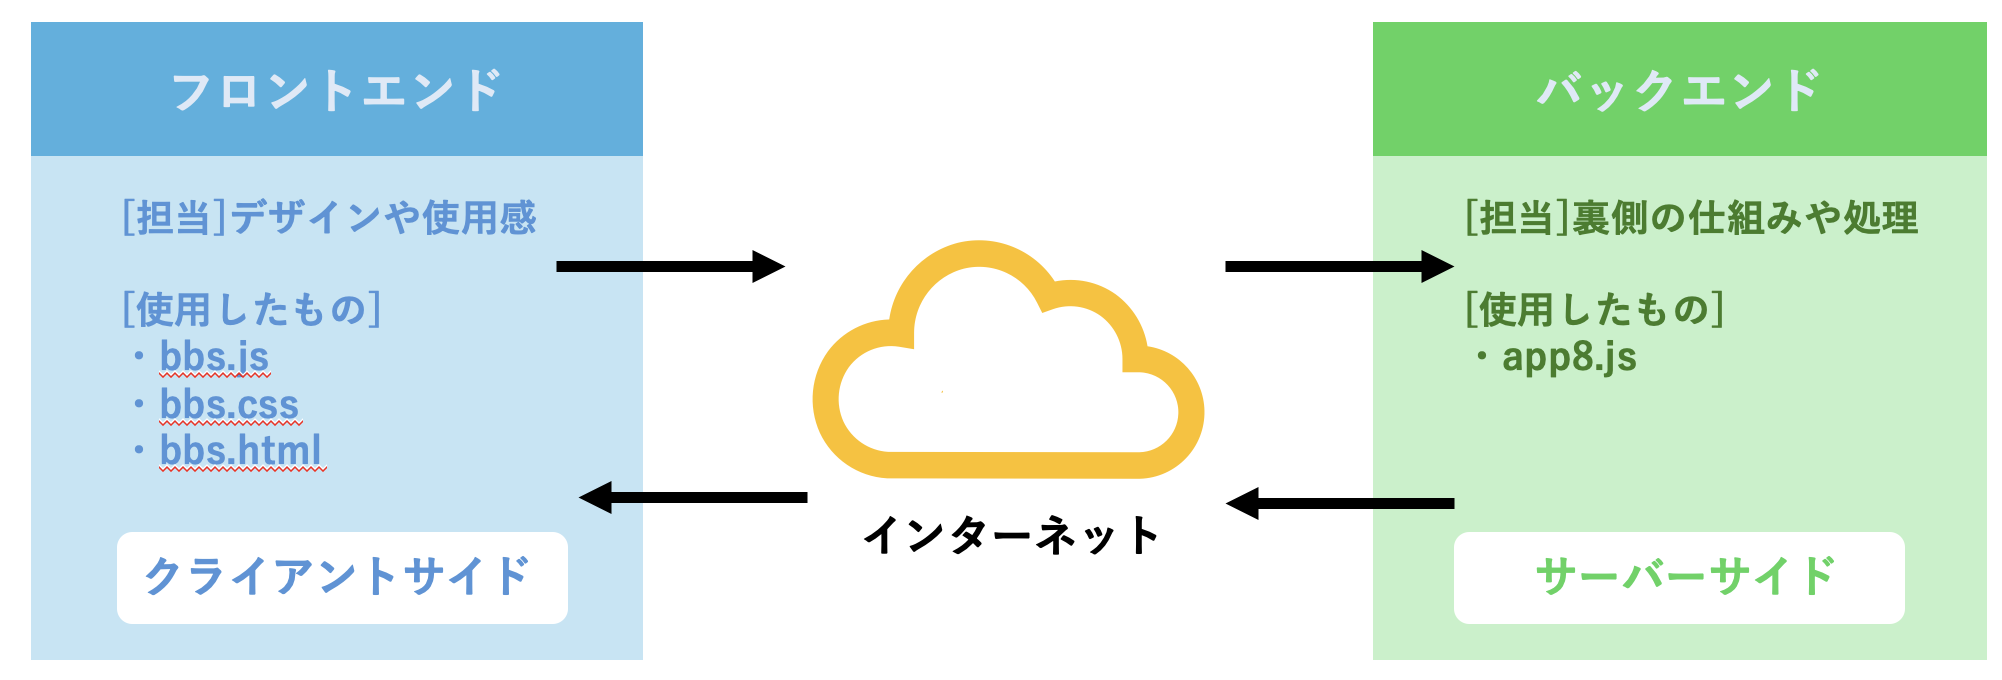
\includegraphics[width=14cm]{1.png}
    \caption{今回使用したプログラムの関係}
    \label{fig:1}
\end{figure}

\subsection{プログラムの役割}
今回作成したプログラムの役割を以下に示す.
\subsubsection{app8.js(バックエンド)}
\begin{itemize}
    \item \textbf{役割}:サーバーを立ち上げ,リクエストを処理する.
    \item 投稿の管理 (POST /post),投稿データの取得 (POST /read),いいね機能 (POST /like) などのエンドポイントを提供.
    \item データはバックエンド内のbbs配列に保存される.
    \item クライアント(フロントエンド)からのリクエストを処理し,レスポンスを返す.
\end{itemize}

\subsubsection{bbs.html(フロントエンドのHTML)}
\begin{itemize}
    \item \textbf{役割}:ウェブページの構造を定義する.
    \item ユーザーが入力するフォームや,投稿一覧の表示部分を構築.
    \item サーバーと通信するためのスクリプト (bbs.js) を読み込む.
    \item htmlだけでは不十分なデザインを取り入れるためにcssを読み込む.
\end{itemize}

\subsubsection{bbs.html(フロントエンドのCSS)}
\begin{itemize}
    \item \textbf{役割}:ウェブページの見た目をデザインする.
    \item フォーム,投稿のリスト,ボタンなどのスタイル(色,フォント,レイアウト)を指定.
\end{itemize}

\subsubsection{bbs.html(フロントエンドのJavaScript)}
\begin{itemize}
    \item \textbf{役割}:ウェブページの動きを制御する.
    \item 取得したデータをHTMLに動的に反映する(例: 投稿リストの表示,いいね数の更新).
\end{itemize}

\section{利用者向け}
以下は,利用者を対象にした仕様書である.
\clearpage
\subsection{掲示板の使い方1}
掲示板の使い方について掲示板の画像をつかって以下で説明する.
\begin{figure}[h]
    \centering
    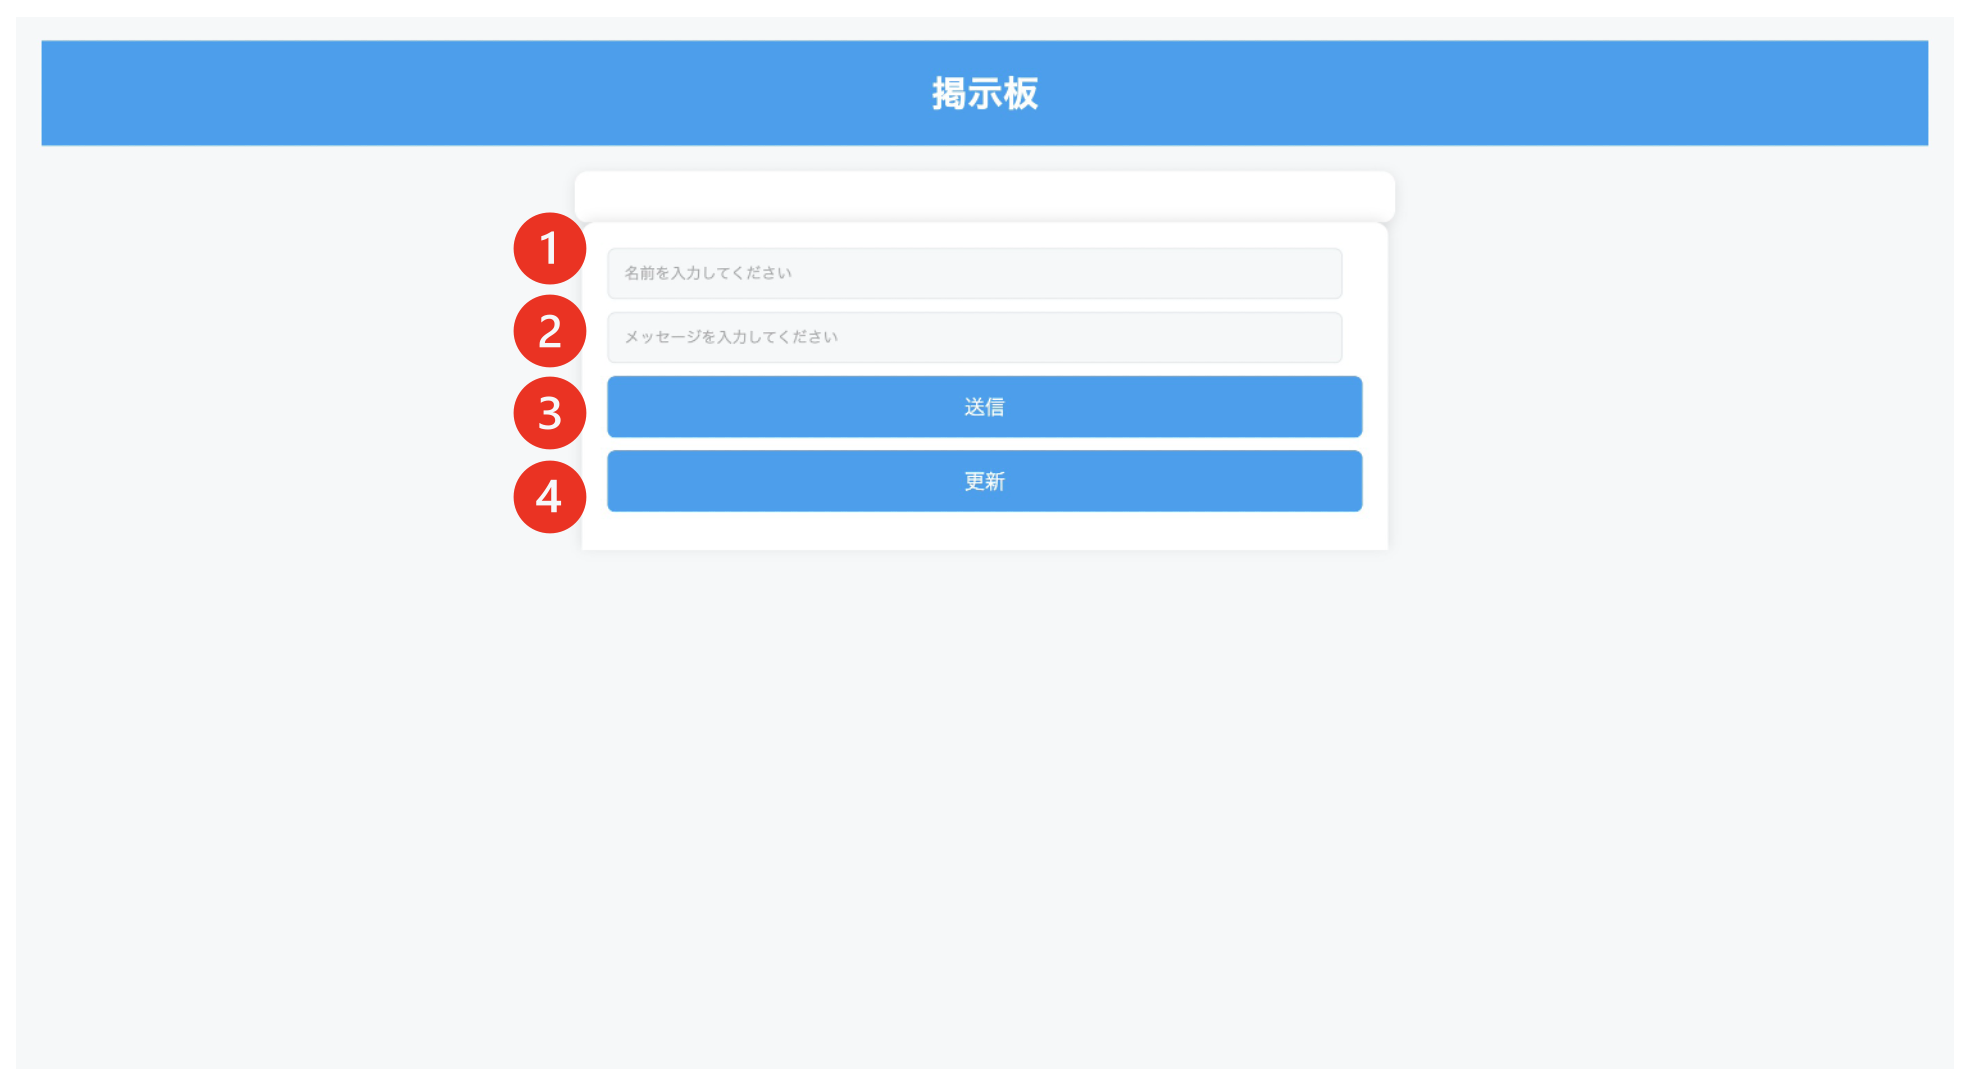
\includegraphics[width=14cm]{使用者2.png}
    \caption{使用方法1}
    \label{fig:使用者1}
\end{figure}

掲示板の基本的な操作手順は,以下の通りである.
\begin{enumerate} 
    \item 名前を入力する.
    \item メッセージを入力する.
    \item 送信ボタンを押す.
    \item 更新ボタンを押し,内容を反映させる.
\end{enumerate} 
また,メッセージを入力しなくても,他のユーザーが入力したメッセージがあれば,更新ボタンを押すことでその内容が反映される.

\clearpage
\subsection{掲示板の使い方2}
次に掲示板で使用できる機能を掲示板の画像を用いて以下で説明する.

\begin{figure}[h]
    \centering
    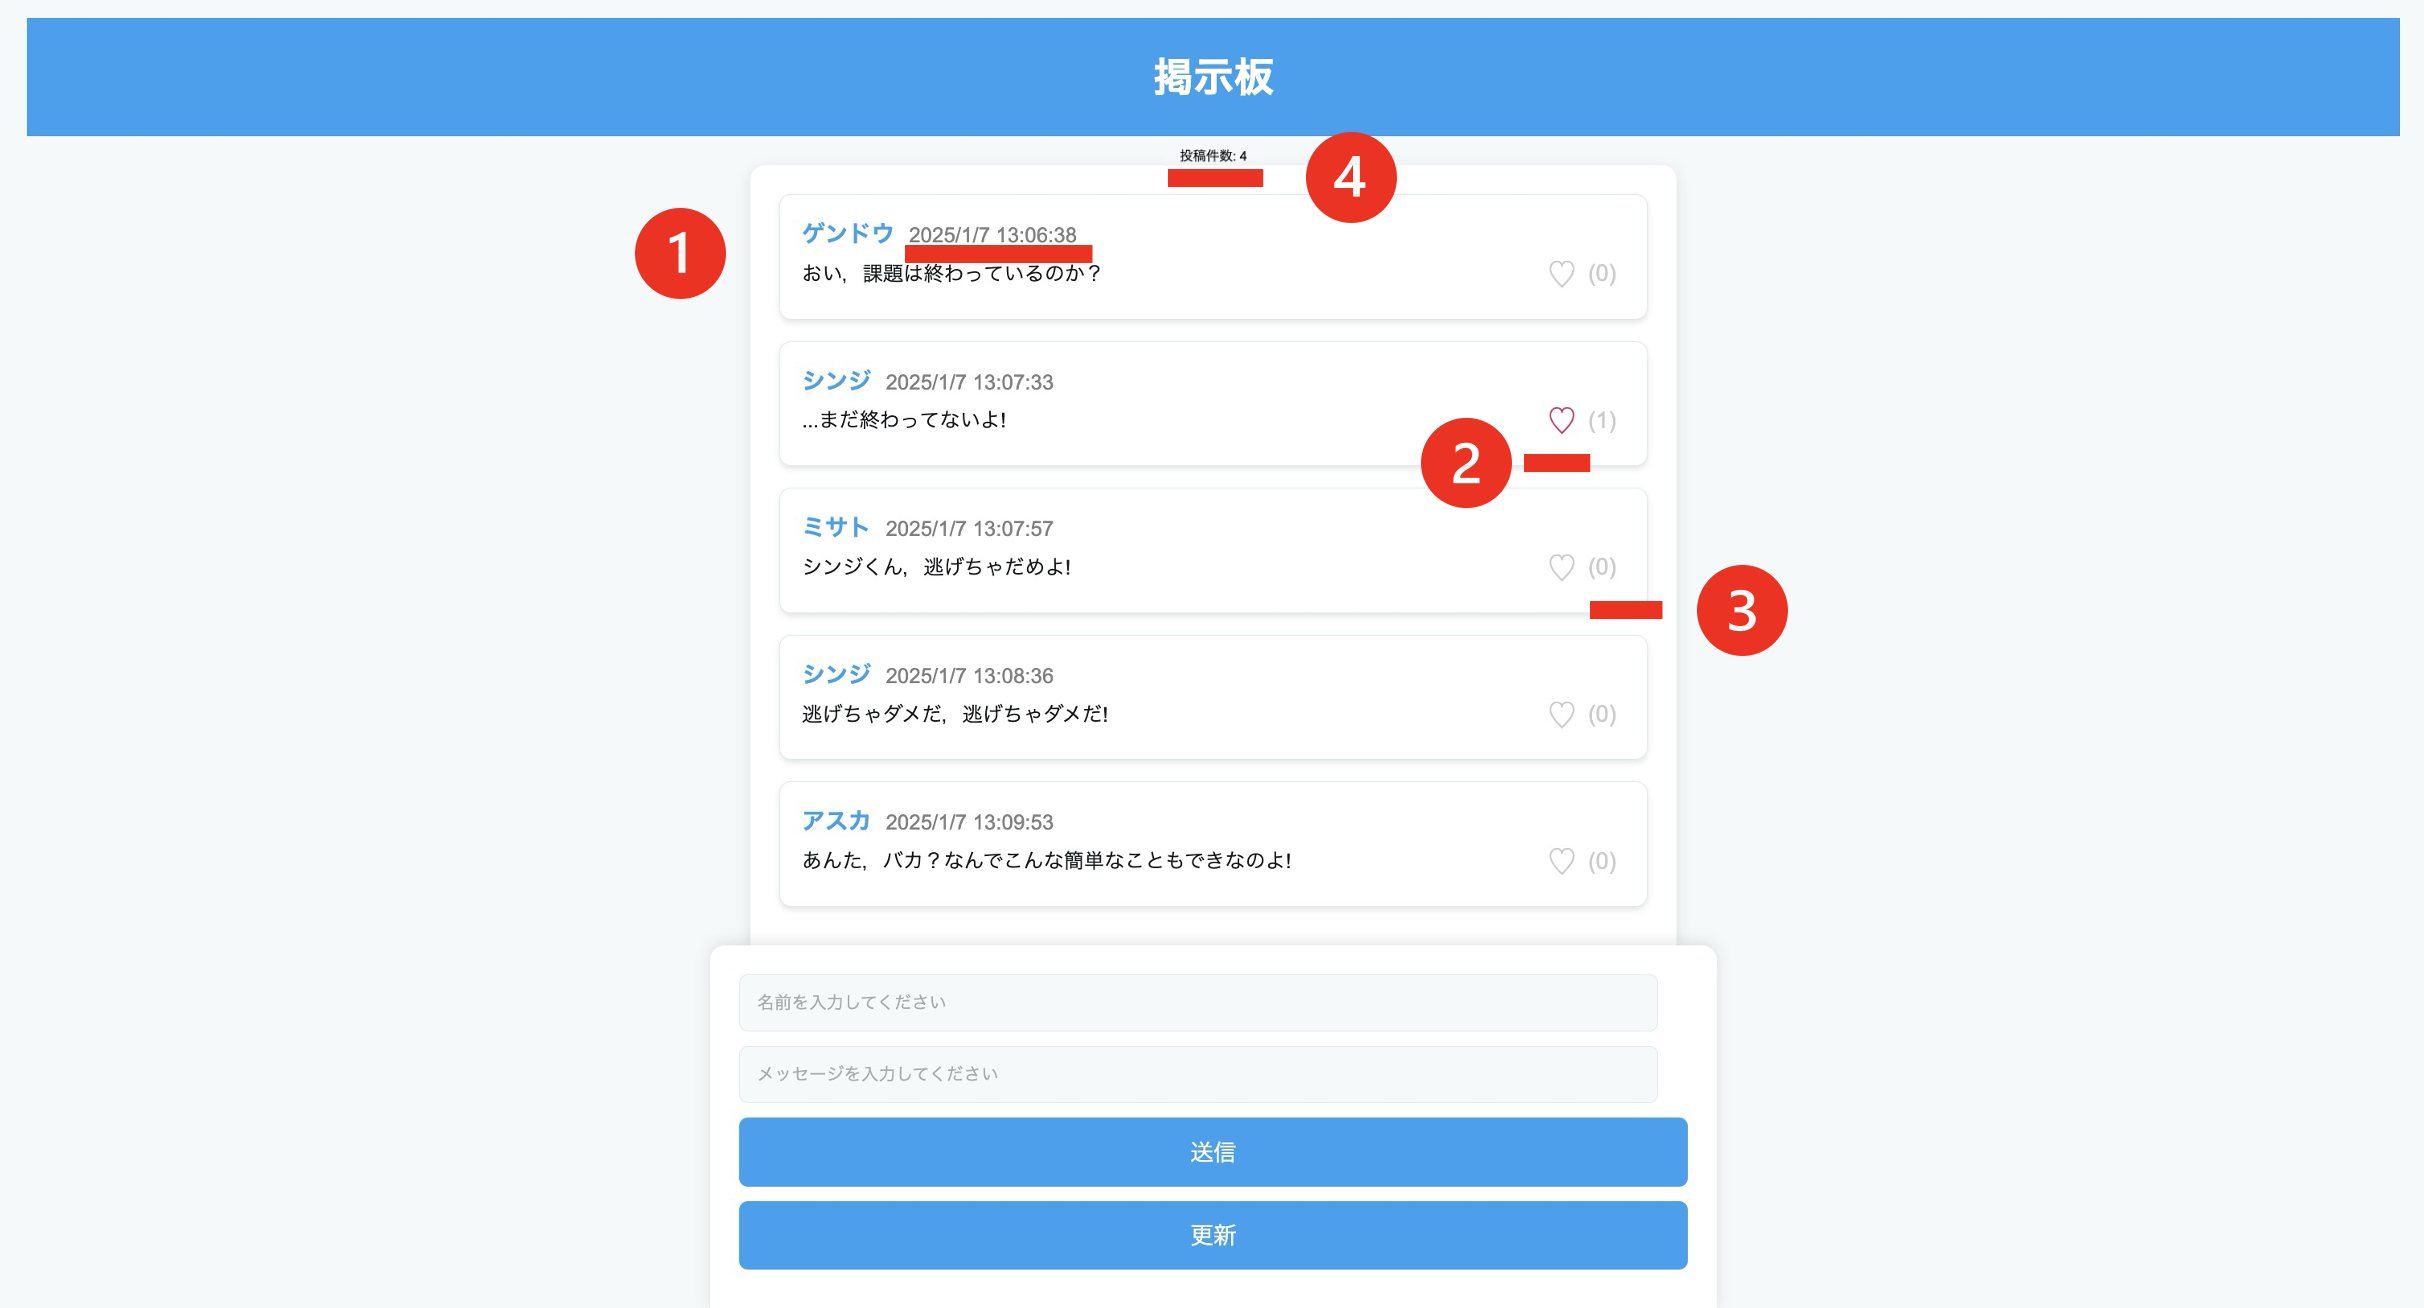
\includegraphics[width=14cm]{使用者3.png}
    \caption{使用方法2}
    \label{fig:使用者2}
\end{figure}

掲示板の基本的な機能は,以下の通りである.
\begin{enumerate}
    \item \textbf{日付} :送信された時間をweb上で反映させる
    \item \textbf{いいね} :ユーザーがいいねを押すことができる
    \item \textbf{いいねカウント} :ユーザーがいいねを押した回数を記録する
    \item \textbf{投稿件数} :すべてのユーザーが投稿した回数を記録する
\end{enumerate}

\subsection{掲示板の使い方3}
この掲示板は,パソコン,タブレット,スマートフォンなど,さまざまなデバイスに対応している.
\clearpage
\begin{figure}[h]
    \centering
    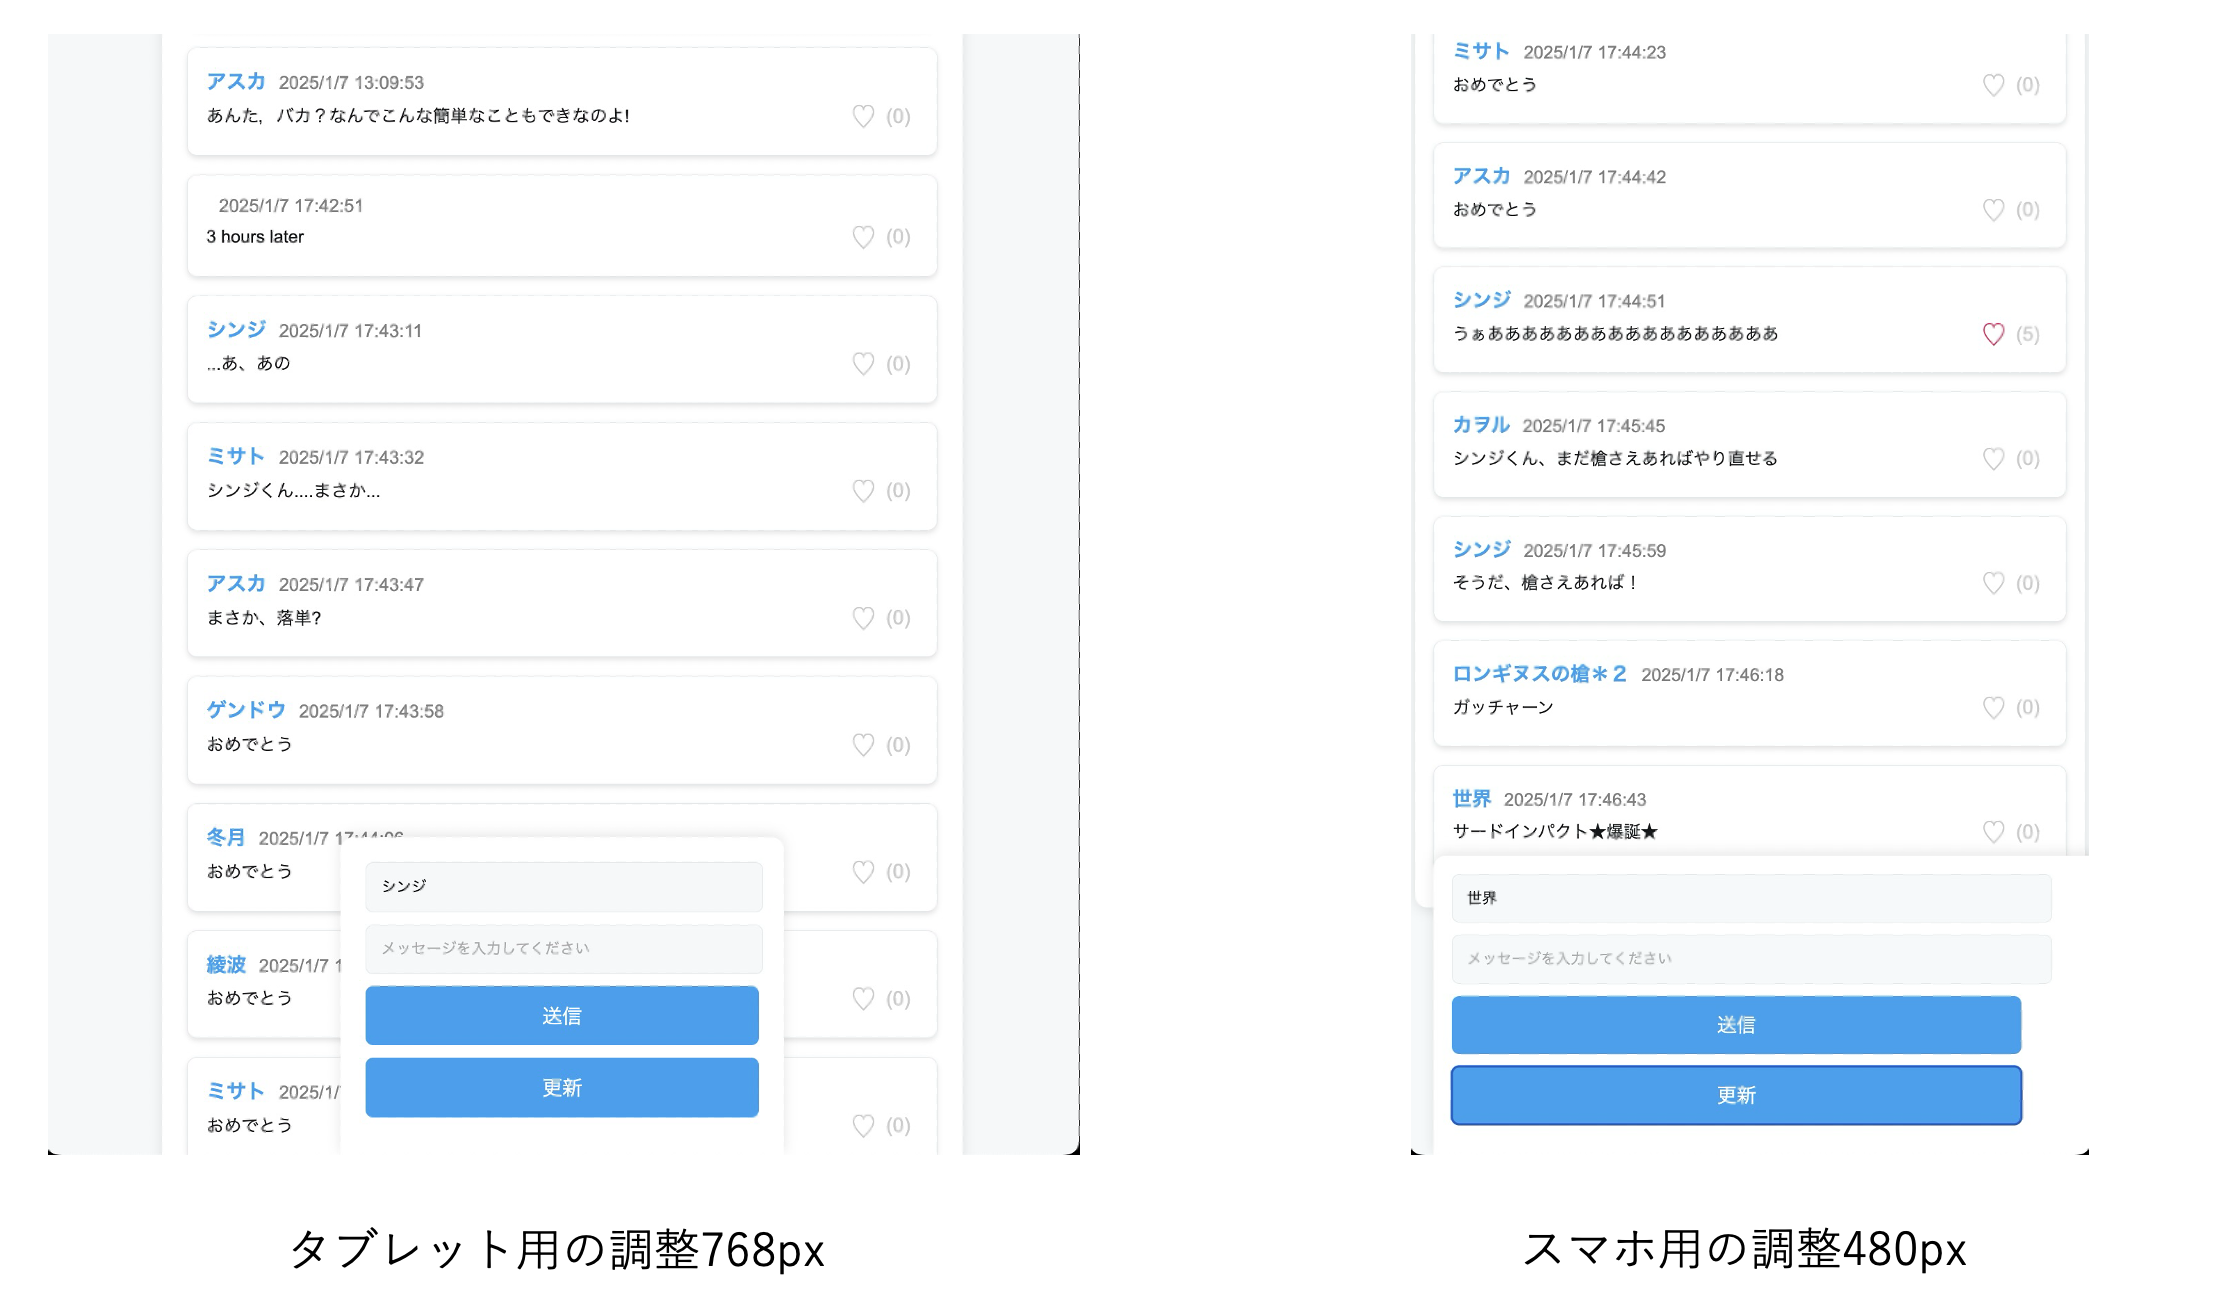
\includegraphics[width=14cm]{使用者4.png}
    \caption{使用方法3}
    \label{fig:使用者3}
\end{figure}

また,視認性や使いやすさを向上させるためにさらなる機能を追加している.

\begin{figure}[h]
    \centering
    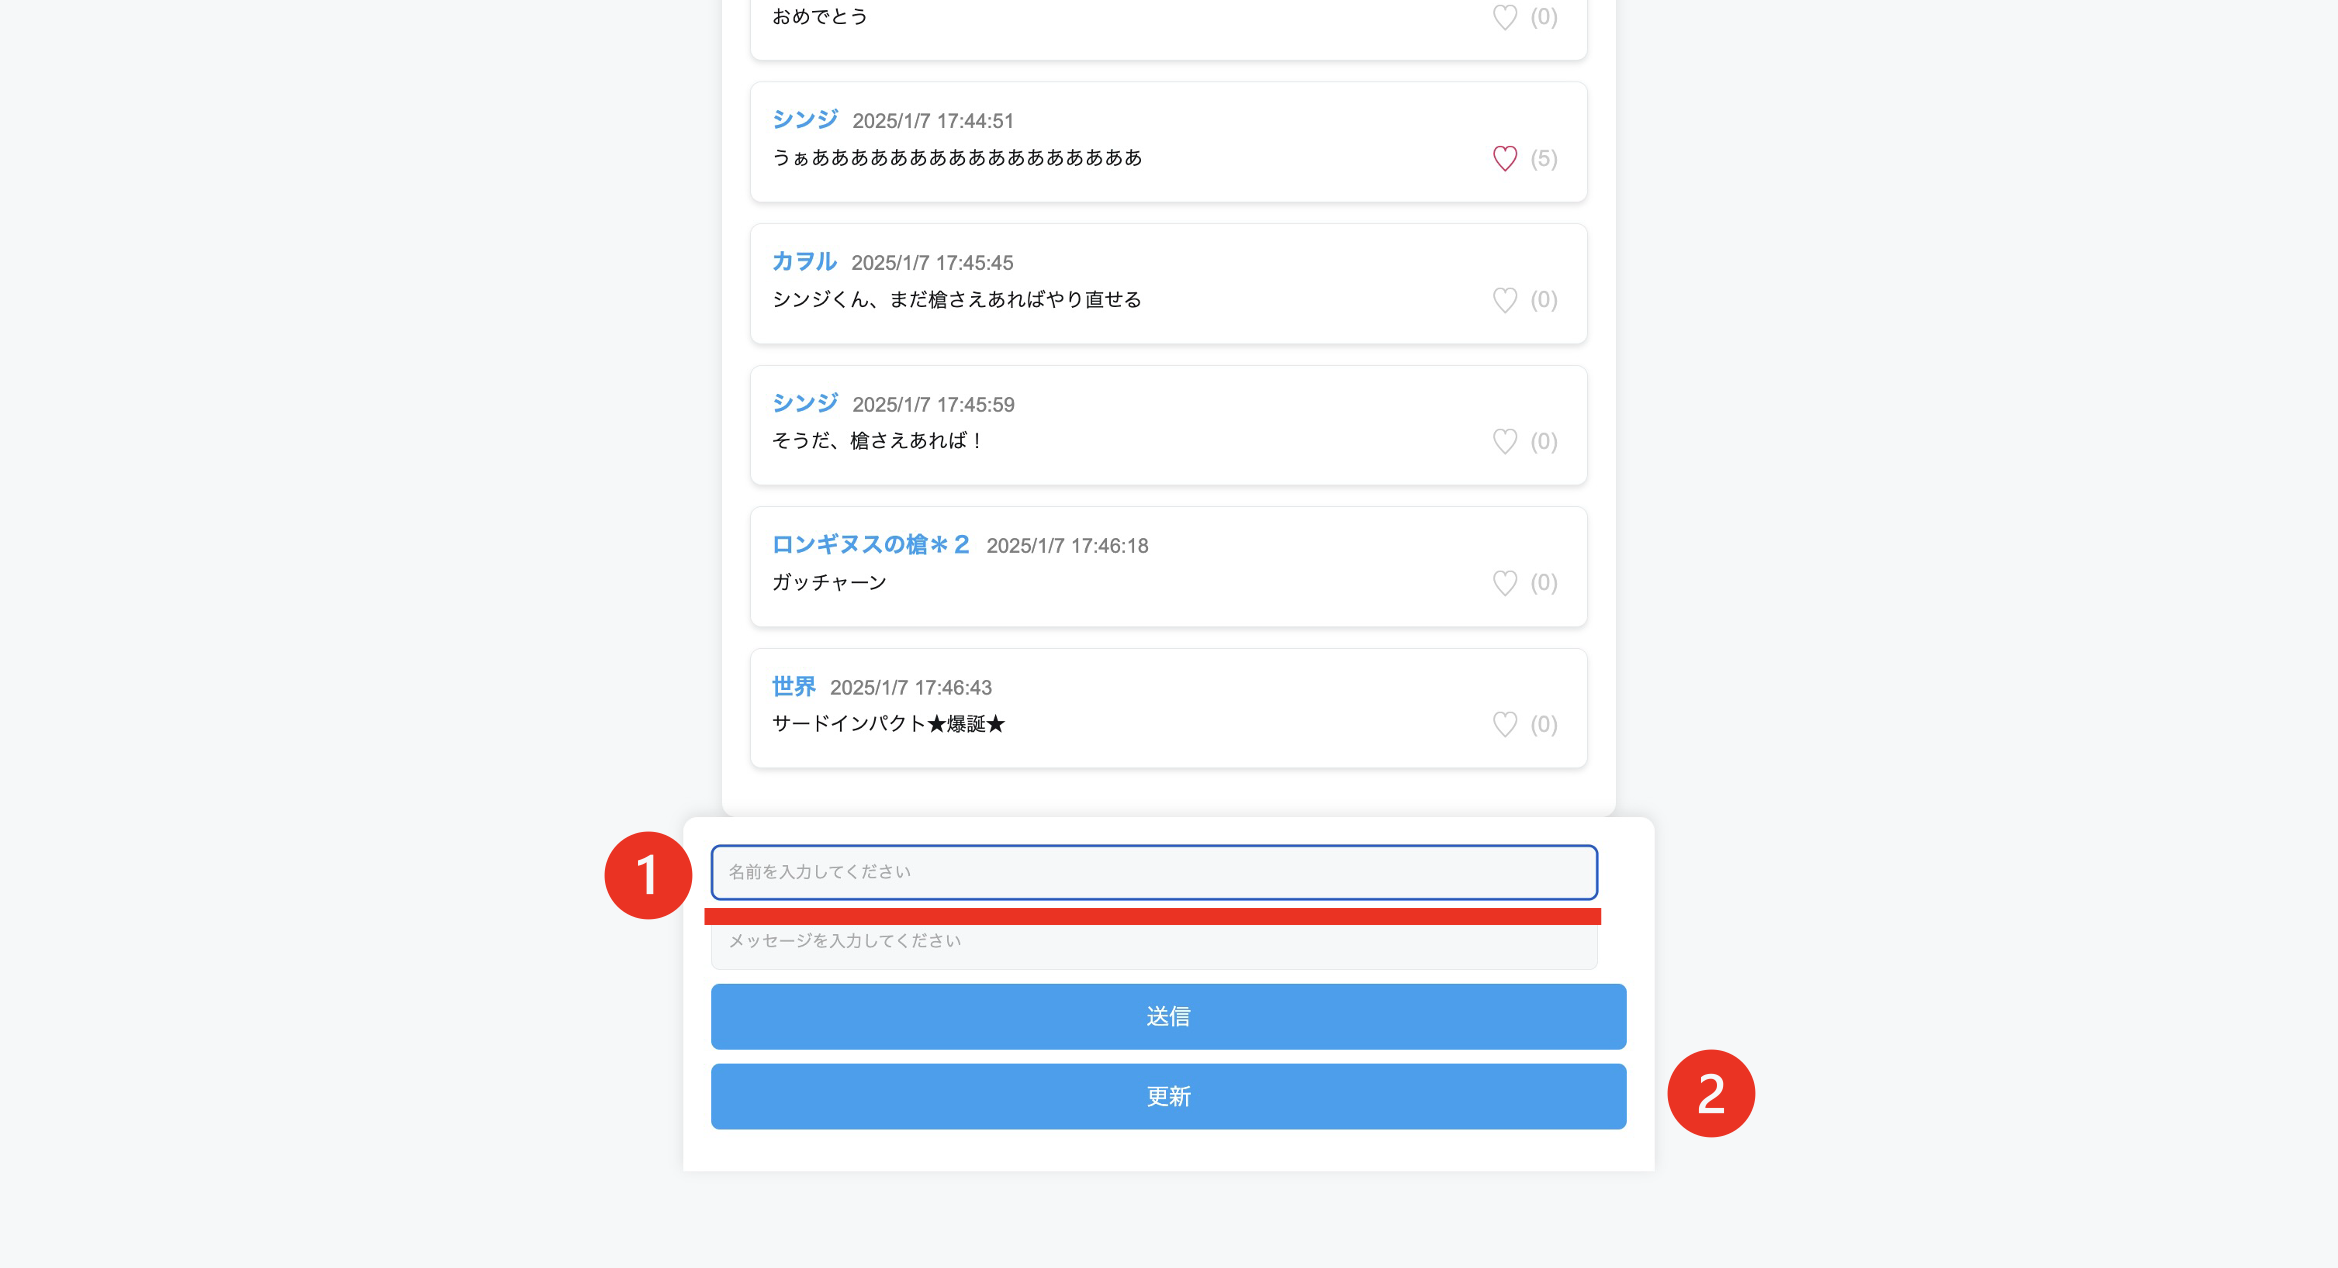
\includegraphics[width=14cm]{使用者5.png}
    \caption{使用方法4}
    \label{fig:使用者4}
\end{figure}

\begin{enumerate}
    \item \textbf{フォーム枠} :選択時に濃い青い枠が表示される
    \item \textbf{固定スクロール} :スクロールしても入力フォームが常に画面下部に固定されている
\end{enumerate}



\clearpage
\section{管理者向け}
以下は,管理者を対象にした仕様書である.

\subsection{サーバーの立ち上げ手順}
掲示板で用いるサーバーの立ち上げ方は以下の手順の通りである.

\subsubsection{サーバーの立ち上げ}
バックエンド側のサーバー(app8.js)を起動する手順は次の通りである.
\begin{enumerate}
    \item ターミナルを起動し,サーバー処理をするバックエンド側のJavaScriptファイルがあるディレクトリに移動する.(例:cd /Desktop/webpro/webpro\_06)
    \item 今回は app8.js がサーバー処理をするバックエンド側のJavaScriptなので,以下のコマンドを実行する.node app8.js
\end{enumerate}

\subsubsection{telnetによるサーバー接続}
別のターミナルを立ち上げて,telnetを使用してサーバーに接続する手順は次の通りである.
\begin{enumerate} 
    \item ターミナルを起動し,以下のコマンドを実行する.\\
    telnet localhost 8080
    \item 接続が成功したら,以下のコマンドを順に実行する.
    \begin{enumerate} 
        \item HTTPリクエストの開始行を入力する.\\
        GET /bbs HTTP/1.1
        \item 次に,ホスト名を指定する.\\
        Host: localhost
    \end{enumerate} 
    \item 最後に,空行(Enterキーを2回押す)を送信してリクエストを終了する. 
\end{enumerate}

\clearpage
\subsection{ログの出力形式及びログの見方}
サーバーの動作ログは基本的に以下の通りである.
\begin{enumerate}
    \item \textbf{起動時} :Example app listening on port 8080!
    \item \textbf{投稿取得時} :GET /BBS
    \item \textbf{各投稿データ} :[ 'name:', 'ゲンドウ', 'message:', 'おい,課題は終わっているのか?', 'date', '2025/1/7 13:06:38' ]
    \item \textbf{読み取られた順序} :read -$>$ X
\end{enumerate}

\begin{figure}[h]
    \centering
    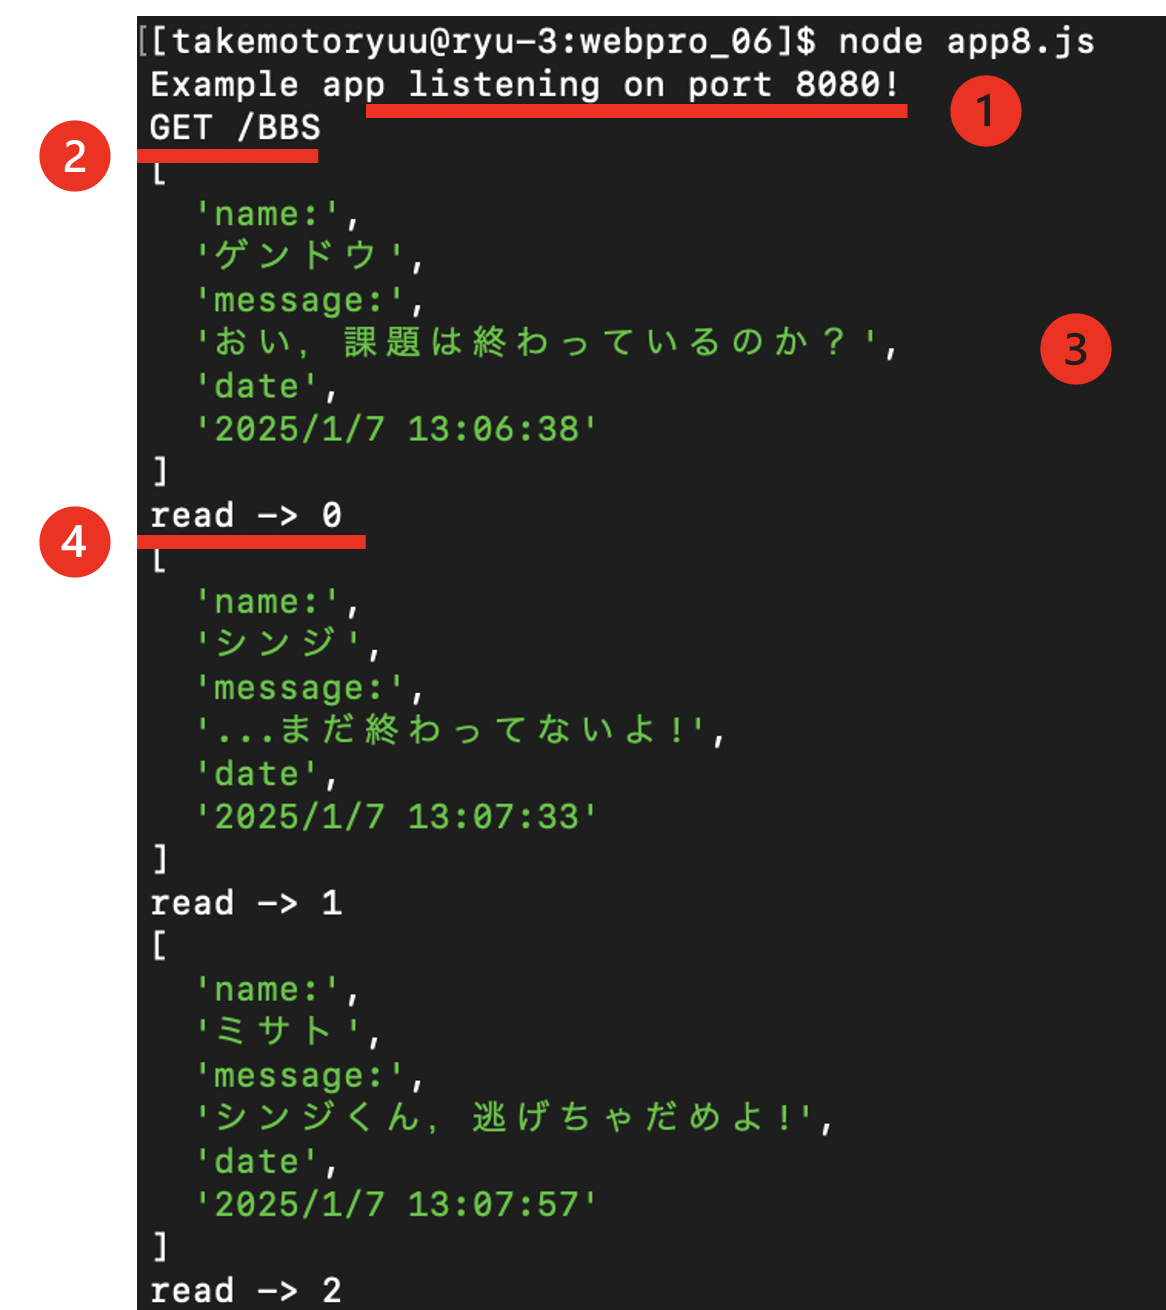
\includegraphics[width=12cm]{管理者2.png}
    \caption{管理者}
    \label{fig:管理者}
\end{figure}

サーバーの動作ログを確認にすることで,投稿者の名前,投稿内容,投稿日時からスパム投稿や不適切な投稿の特定に役立てることができる.


\clearpage
\section{開発者向け}
以下は,開発者を対象にした仕様書である.以下の3つについて詳しく解説する.
\begin{itemize}
    \item \textbf{「送信」ボタンがクリックされた時の処理 (POST /post)}
    \item \textbf{「更新」ボタンがクリックされた時の処理 (POST /check → POST /read)}
    \item \textbf{「いいね」ボタンがクリックされた時の処理 (POST /like)}
    \item \textbf{「日付」の処理 (POST /post → POST /check → POST /read)}
    \item \textbf{「投稿件数」の処理 (POST /post → POST /check)}
\end{itemize}

\subsection{「送信」ボタンがクリックされた時の処理}
\begin{itemize}
    \item \textbf{役割}:現在の掲示板の投稿数を確認する.
    \item クライアント側では,投稿数の変化があれば新しい投稿をサーバーから取得し,表示する処理を行う.
\end{itemize}

\begin{figure}[h]
    \centering
    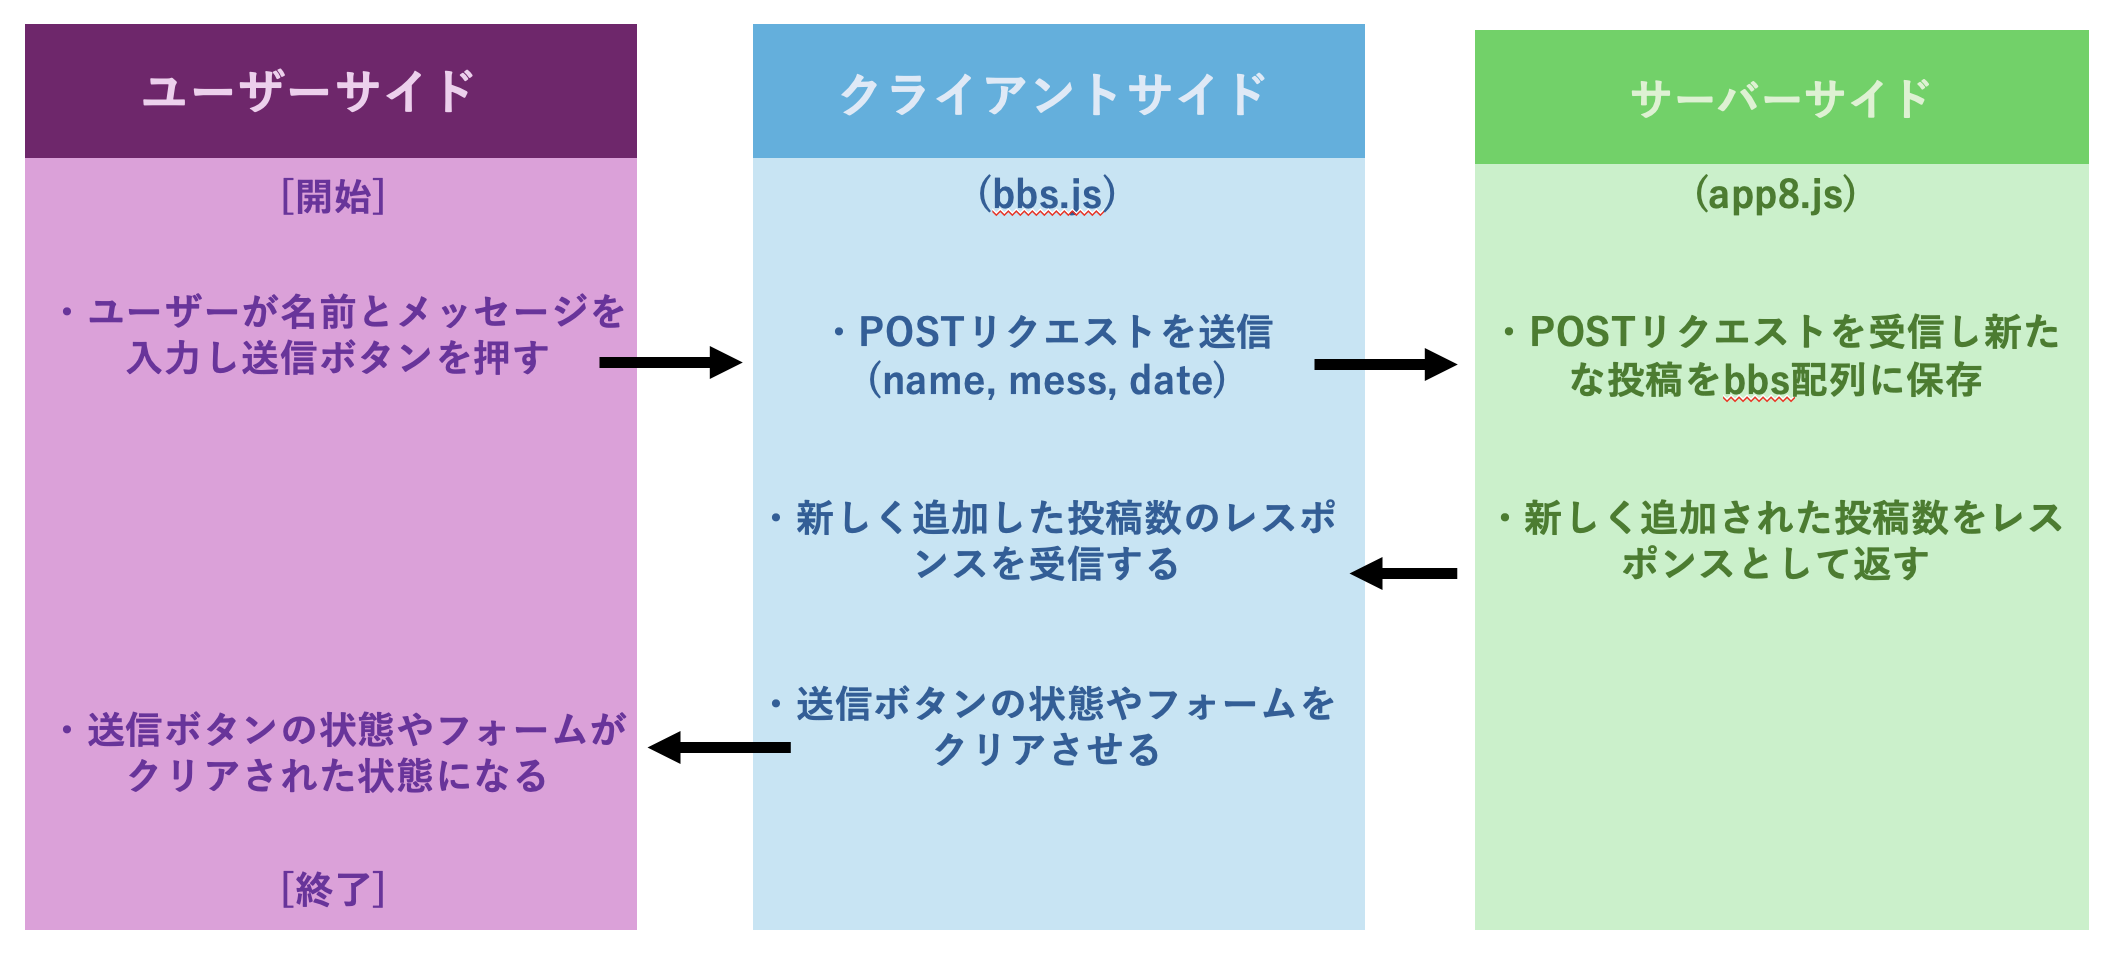
\includegraphics[width=14cm]{送信.png}
    \caption{送信}
    \label{fig:送信}
\end{figure}

\clearpage
\subsection{「更新」ボタンがクリックされた時の処理}
\begin{itemize}
    \item \textbf{役割}:現在の掲示板の投稿数を確認し,更新する.
    \item クライアント側では,投稿数の変化があれば新しい投稿をサーバーから取得し,表示する処理を行う.
\end{itemize}

\begin{figure}[h]
    \centering
    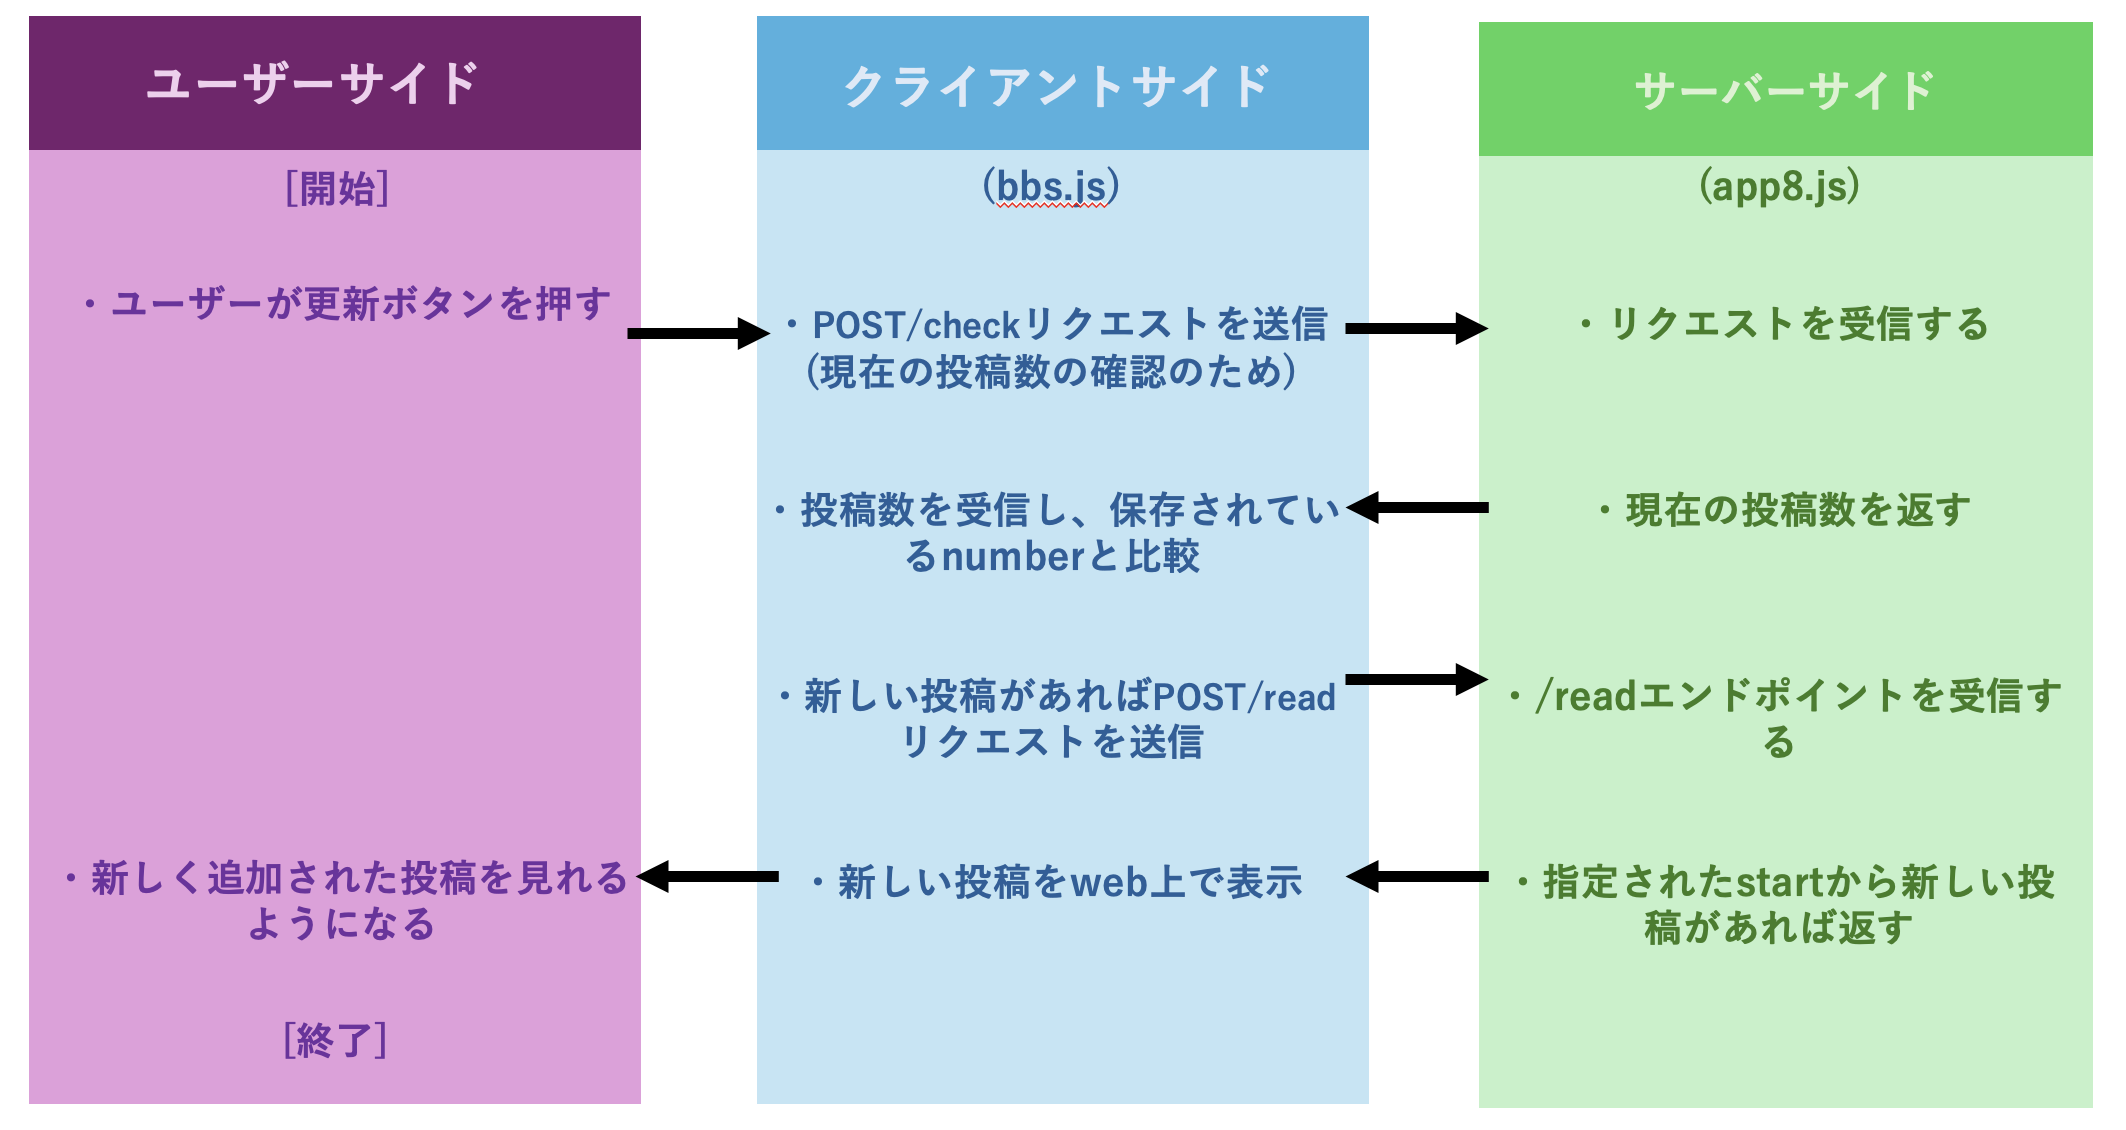
\includegraphics[width=14cm]{更新.png}
    \caption{更新}
    \label{fig:更新}
\end{figure}

\clearpage
\subsection{「いいね」ボタンがクリックされた時の処理}
\begin{itemize}
    \item \textbf{役割}:現在の掲示板のいいね数を確認し,一つ一つの投稿に紐づけられたpostIdを用いて,いいね数を増加させる.
    \item クライアント側では,ユーザー側に新しい投稿があればサーバーから取得し,表示する処理を行う.
    \item サーバー側では,bbs配列内の該当するIdを取得し,いいね数を増加させてレスポンスする.
\end{itemize}

\begin{figure}[h]
    \centering
    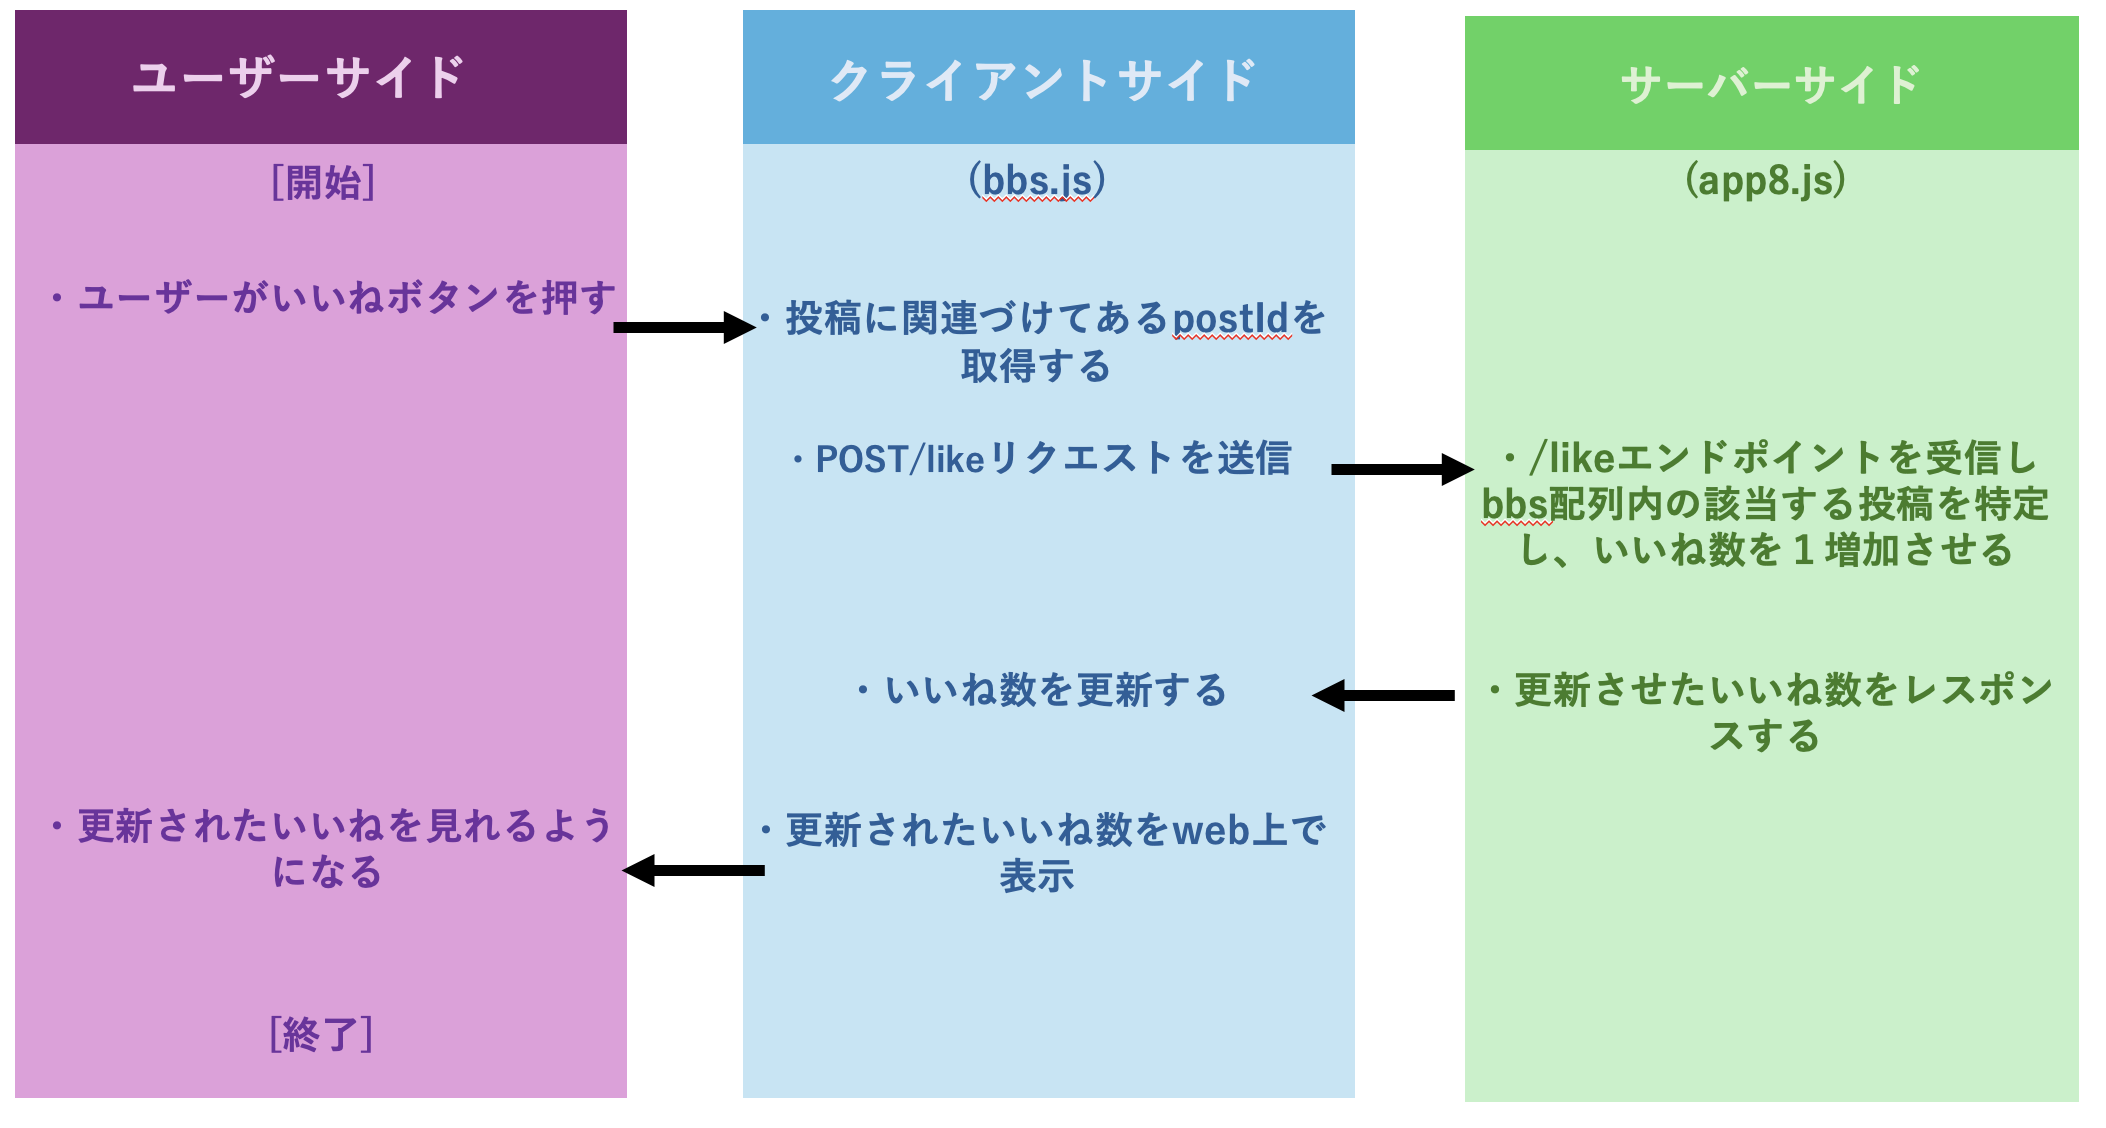
\includegraphics[width=14cm]{いいね.png}
    \caption{いいね}
    \label{fig:いいね}
\end{figure}

\clearpage
\subsection{「日付」の処理}
app8.jsのapp.post("/post")で使用しているが,
JavaScriptでは,new Date()で現在日時を取得でき,その後ろに.toLocaleString()と記入すると,数値を日本のローカルに適した数値表示をすることができる.

\begin{figure}[h]
    \centering
    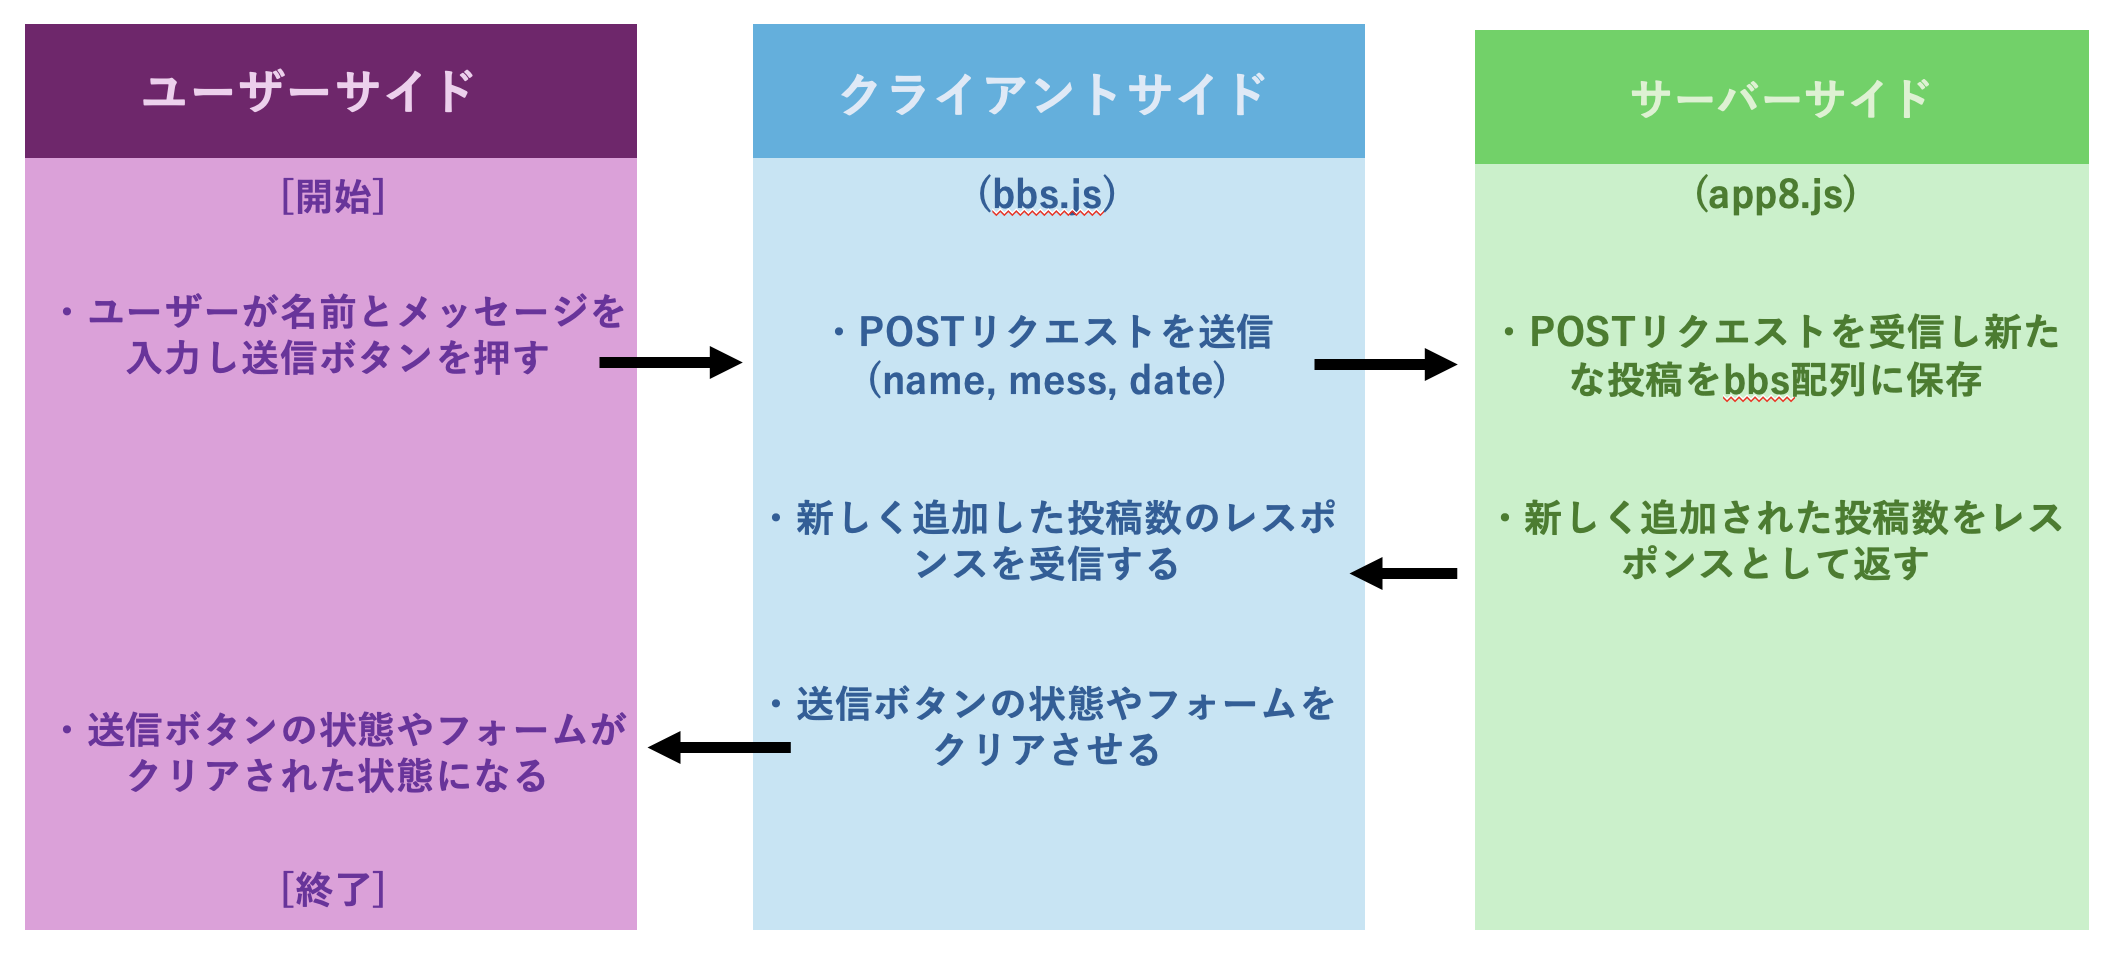
\includegraphics[width=14cm]{送信.png}
    \caption{日付の送信}
    \label{fig:日付の送信}
\end{figure}

\begin{figure}[h]
    \centering
    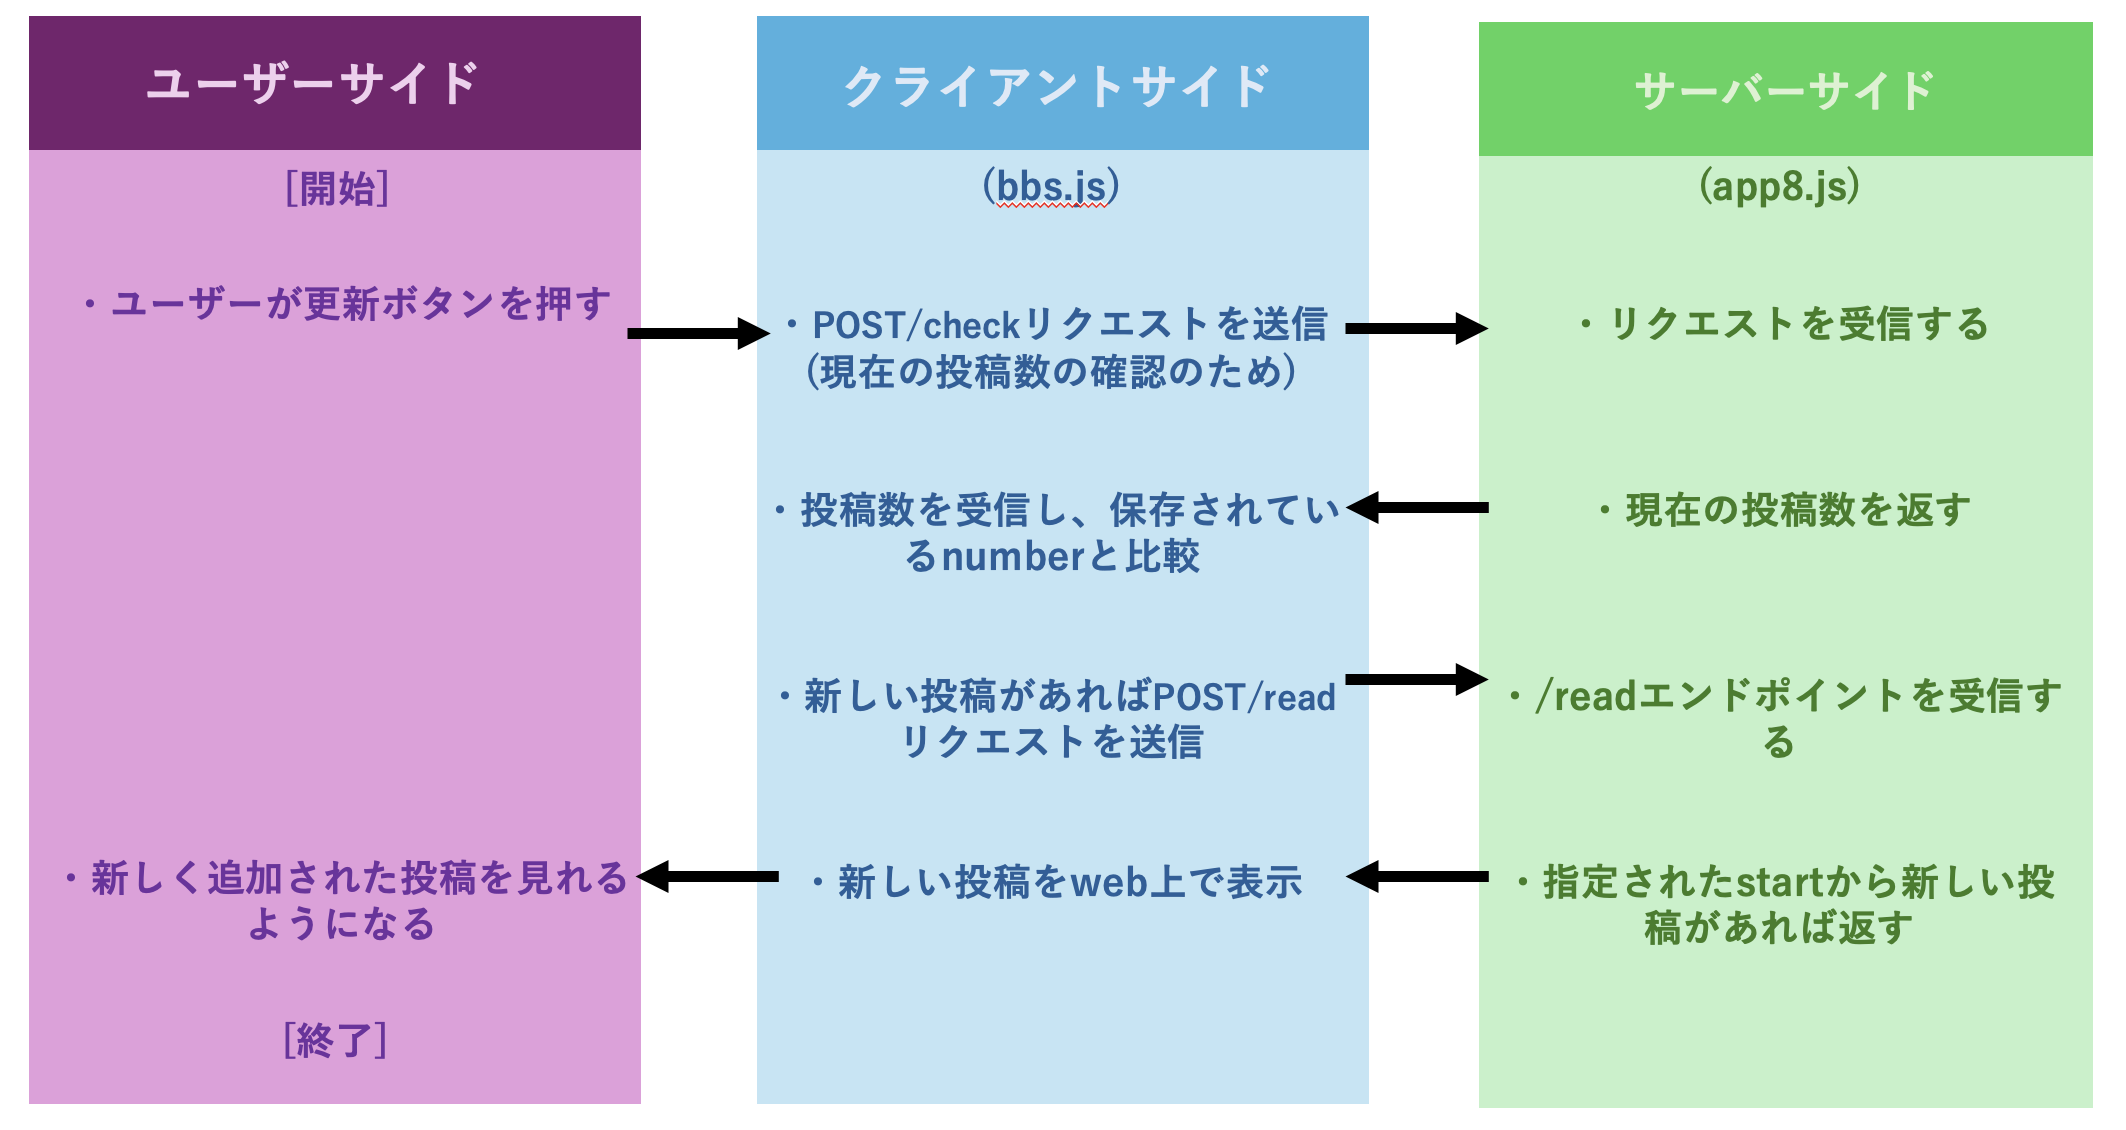
\includegraphics[width=14cm]{更新.png}
    \caption{日付の更新}
    \label{fig:日付の更新}
\end{figure}
日付の更新については,「「送信」ボタンがクリックされた時の処理」及び「「更新」ボタンがクリックされた時の処理」と全く同じである.
\clearpage
\subsection{「投稿件数」の処理}
「投稿件数」の処理について以下に示す.
\begin{figure}[h]
    \centering
    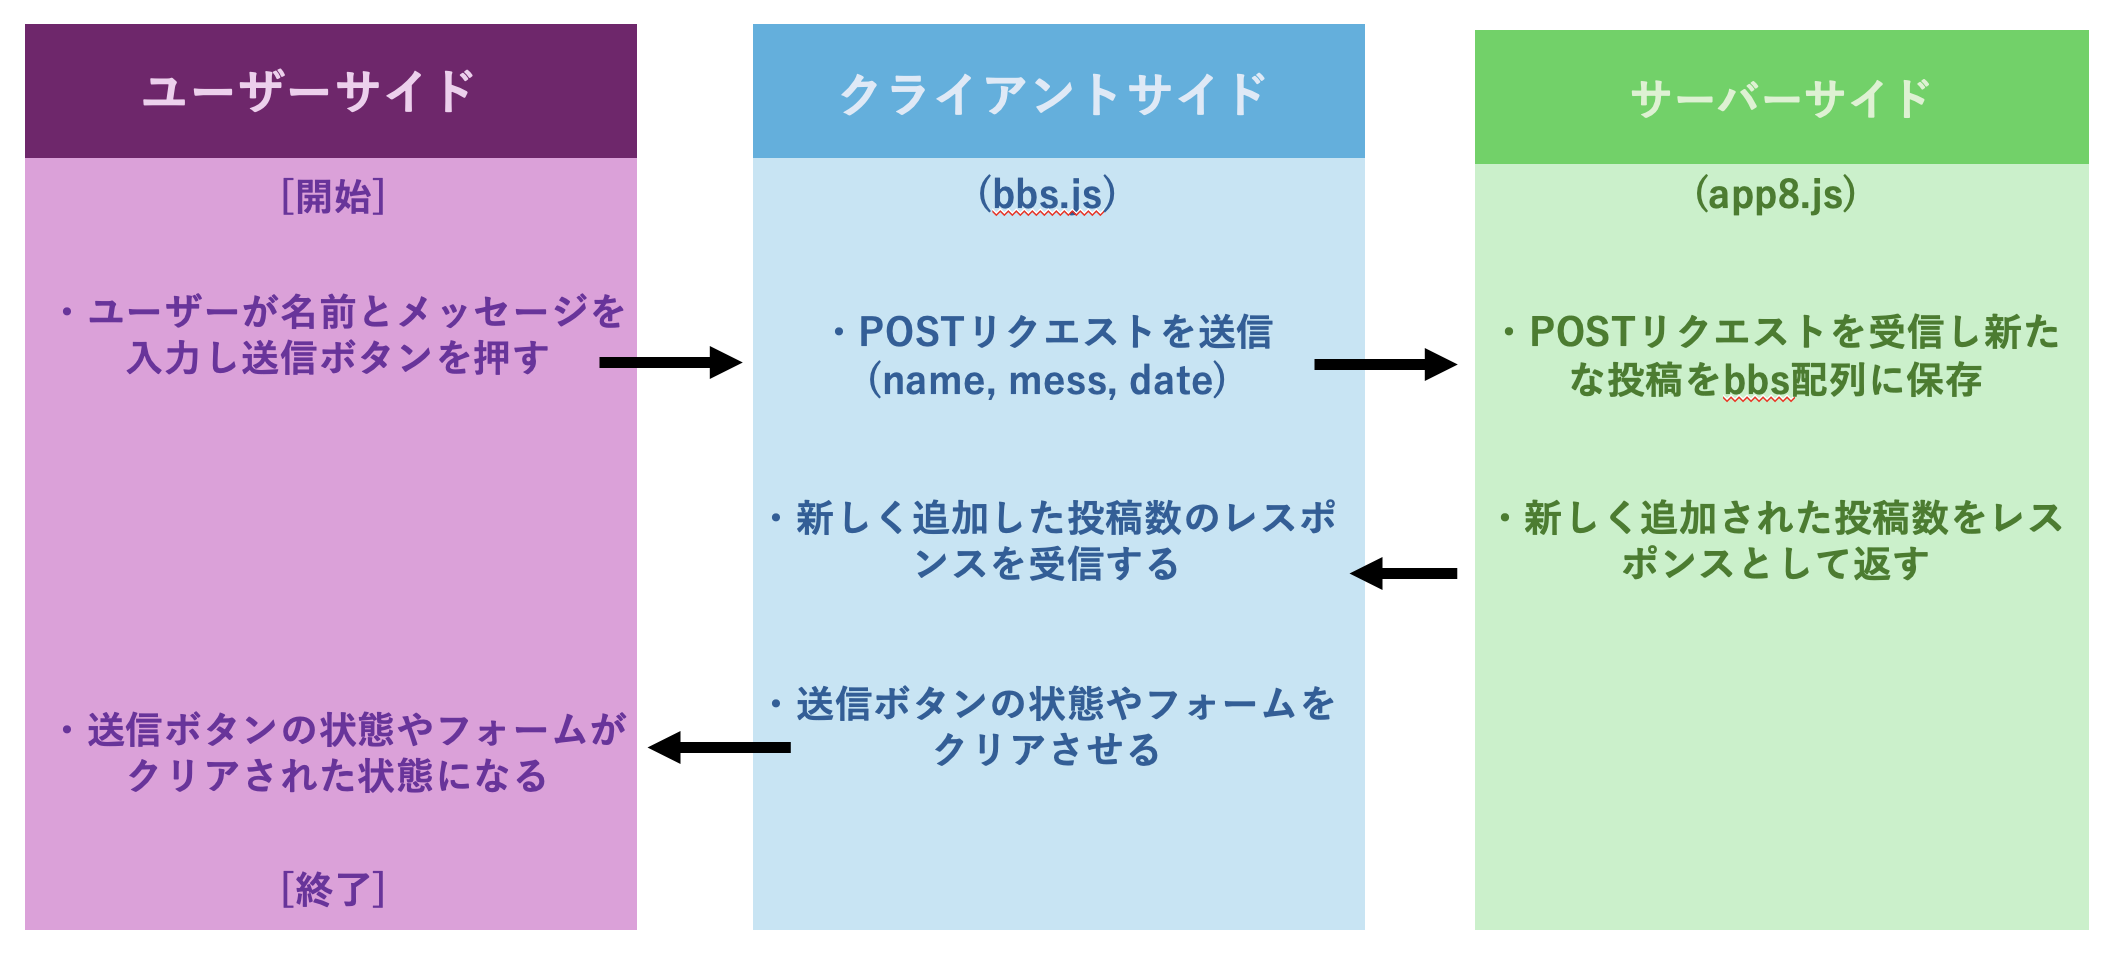
\includegraphics[width=14cm]{送信.png}
    \caption{送信(投稿件数)}
    \label{fig:送信(投稿件数)}
\end{figure}

\begin{figure}[h]
    \centering
    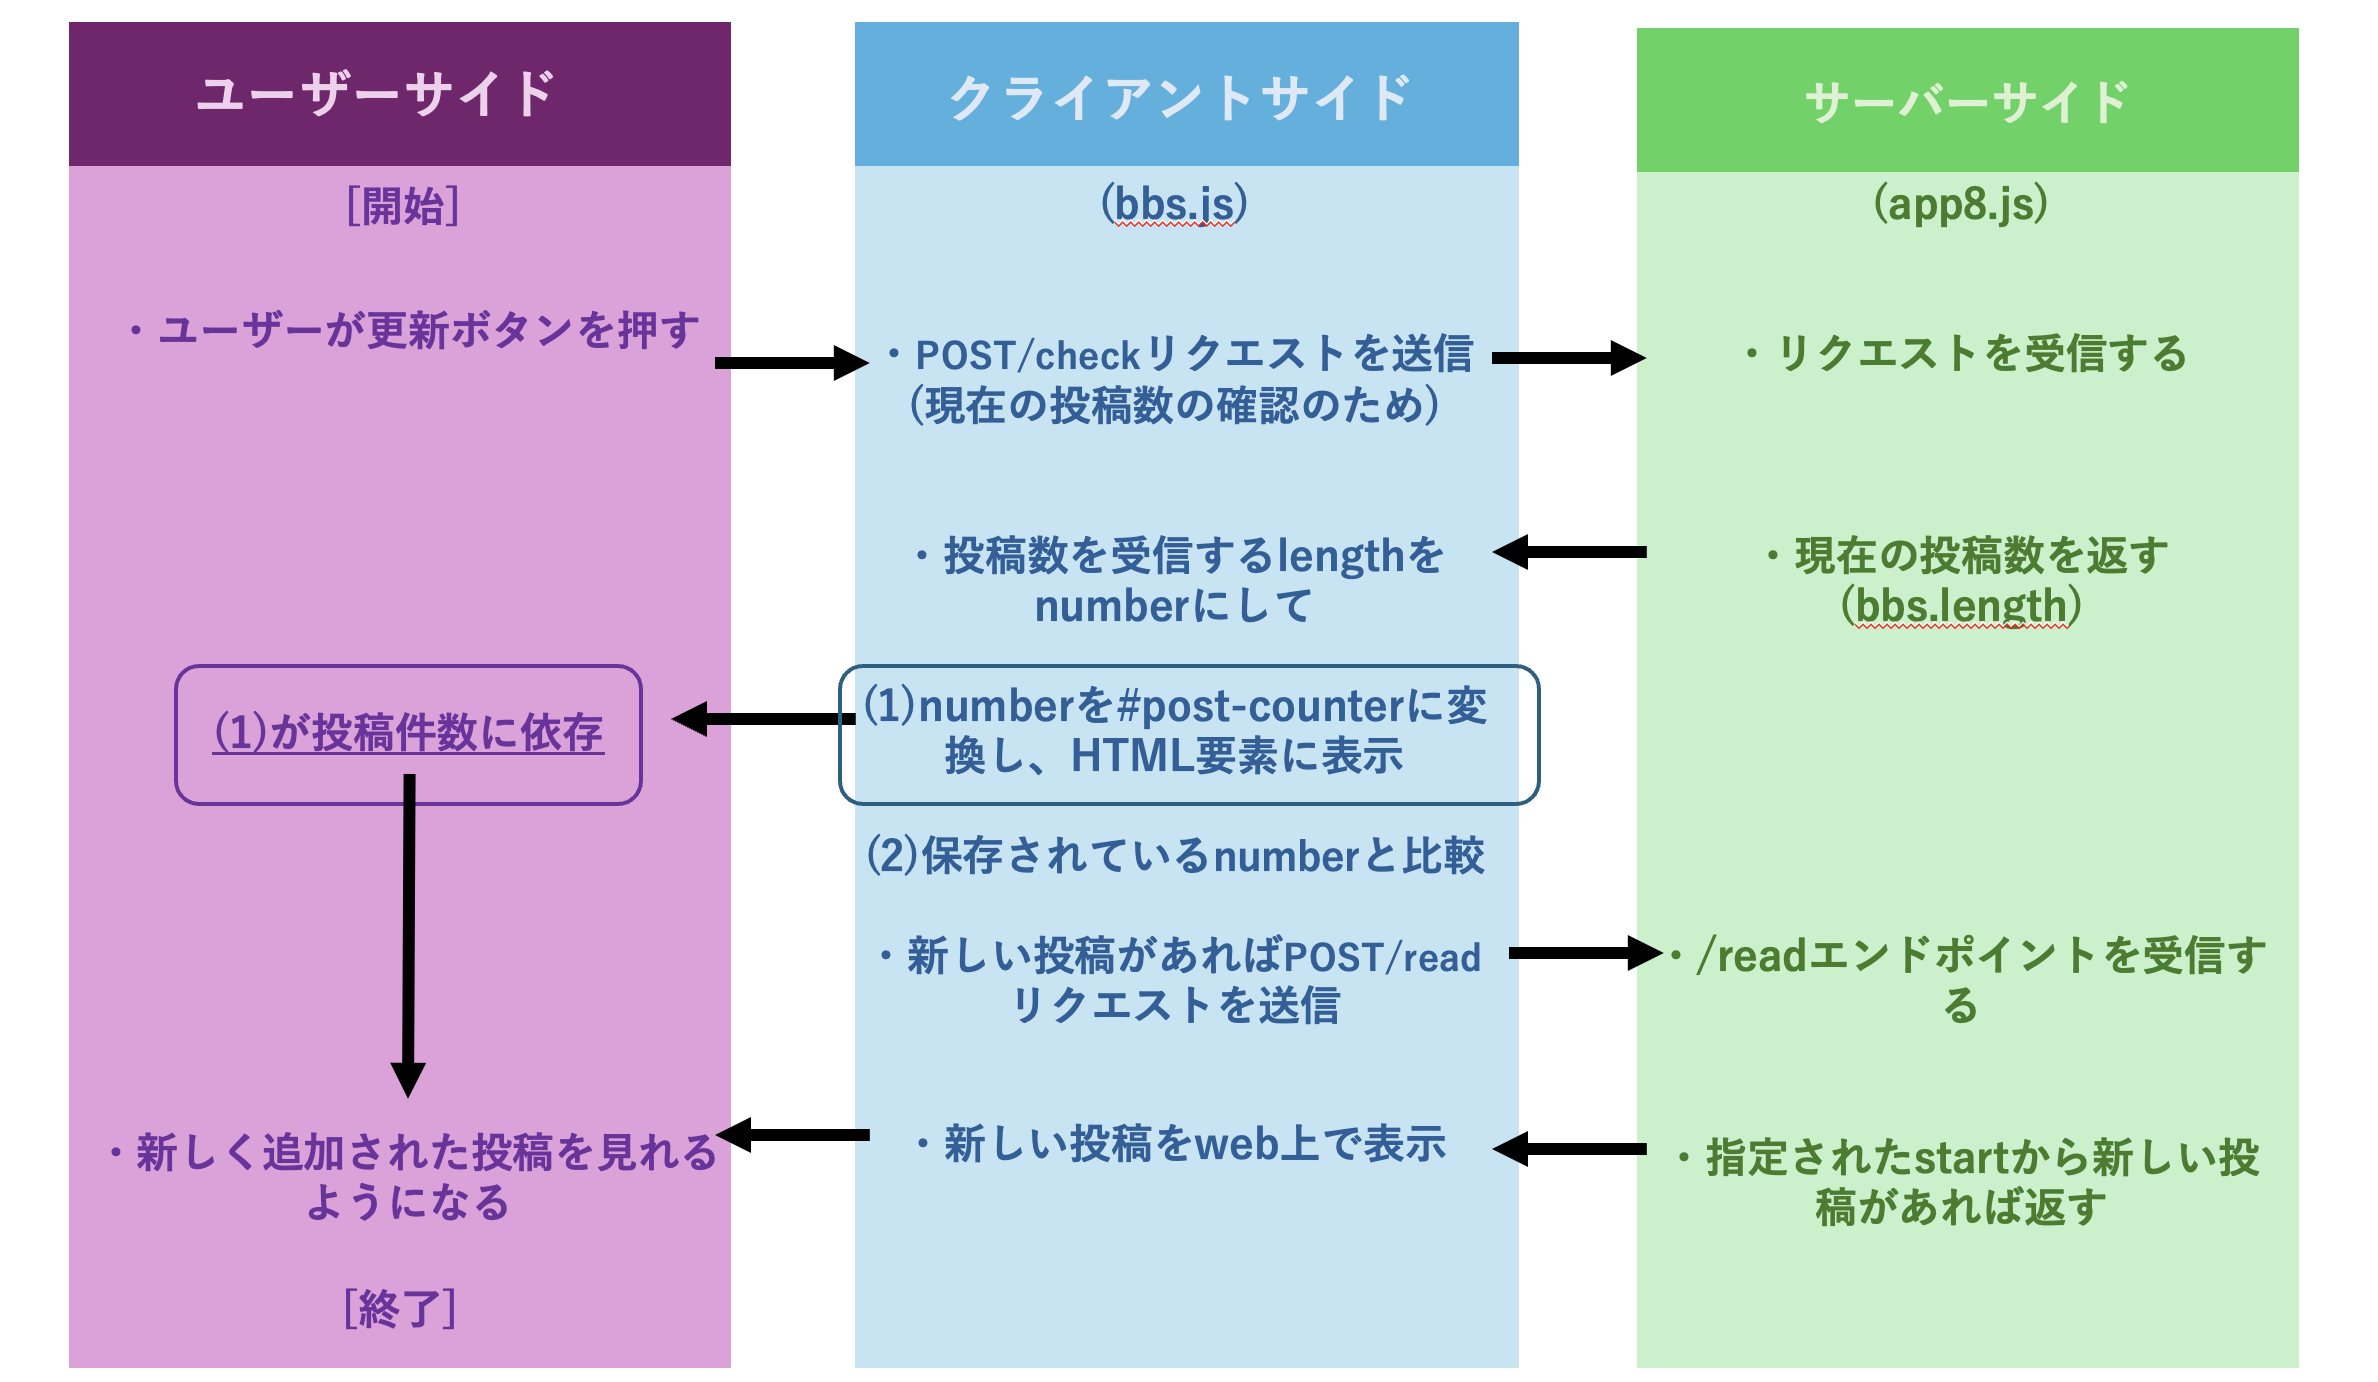
\includegraphics[width=14cm]{更新2.png}
    \caption{更信(投稿件数)}
    \label{fig:更信(投稿件数)}
\end{figure}


「送信」ボタンがクリックされるまでは,「送信」ボタンが押された際の処理が実行される.その後,「更新」ボタンがクリックされた際の処理では,
投稿件数を受信してlengthをnumberに設定する部分までは共通だが,その次の処理が分岐する.(1)の処理は,HTML上に表示された投稿件数に依存するため,
条件を満たさない(2)の処理を行わず,そのまま終了する.

また,app8.js内で,元々あったapp.post("/check")メソッドを使用して,でbbsの配列の長さ(投稿の数)をサーバーからクライアントに送信する.
その際,サーバーから帰ってきたデータをvalueという変数に代入する.その後,

\begin{lstlisting}[firstnumber = 1, caption=valueをpost-countに変換, label=code] 
    document.querySelector('#post-count').innerText = `投稿件数: ${value}`;
\end{lstlisting}

を用いて,HTMLページ上のpost-count変数に数値を代入し,ページ上に投稿件数がリアルタイムで反映できるようにしている.

\clearpage
\section{おわりに}



\section{参考}
\subsection{参考サイト}
\begin{itemize}
    \item https://ics.media/
    \item Chat GPT
    \item YouTube
\end{itemize}

\subsection{参考書籍}
\begin{itemize}
    \item ほんの一手間で劇的に変わるHTML&CSSとWebデザイン実践講座
    \item HTML5&CSS3 デザインブック
\end{itemize}

\end{document}
